%%
%% This is file `elsarticle-template-num.tex',
%% generated with the docstrip utility.
%%
%% The original source files were:
%%
%% elsarticle.dtx  (with options: `numtemplate')
%% 
%% Copyright 2007, 2008 Elsevier Ltd.
%% 
%% This file is part of the 'Elsarticle Bundle'.
%% -------------------------------------------
%% 
%% It may be distributed under the conditions of the LaTeX Project Public
%% License, either version 1.2 of this license or (at your option) any
%% later version.  The latest version of this license is in
%%    http://www.latex-project.org/lppl.txt
%% and version 1.2 or later is part of all distributions of LaTeX
%% version 1999/12/01 or later.
%% 
%% The list of all files belonging to the 'Elsarticle Bundle' is
%% given in the file `manifest.txt'.
%% 

%% Template article for Elsevier's document class `elsarticle'
%% with numbered style bibliographic references
%% SP 2008/03/01

%\documentclass[preprint,12pt]{elsarticle}
%\documentclass[preprint,10pt]{elsarticle}
\documentclass[final,3p,times]{elsarticle} 

%% Use the option review to obtain double line spacing
%% \documentclass[authoryear,preprint,review,12pt]{elsarticle}

%% Use the options 1p,twocolumn; 3p; 3p,twocolumn; 5p; or 5p,twocolumn 

%% for a journal layout:
%% \documentclass[final,1p,times]{elsarticle}
%% \documentclass[final,1p,times,twocolumn]{elsarticle}
%% \documentclass[final,3p,times]{elsarticle}
%% \documentclass[final,3p,times,twocolumn]{elsarticle}
%% \documentclass[final,5p,times]{elsarticle}
%% \documentclass[final,5p,times,twocolumn]{elsarticle}
%
%  various packages that you may wish to activate for usage 
\usepackage{graphics}
\usepackage{graphicx}
\usepackage{tabls}
\usepackage{afterpage}
%\usepackage{cites}
\usepackage{color}
\usepackage{color}

% My standard Packages
%% The amssymb package provides various useful mathematical symbols 
%% The amsthm package provides extended theorem environments
\usepackage{amssymb}
\usepackage{amsmath}
% more math
\usepackage{amsfonts}
\usepackage{amssymb}
\usepackage{amstext}
\usepackage{amsbsy}

\usepackage{subfigure}
\usepackage{multirow}
\usepackage{caption}
	
\usepackage{lscape}

% \journal{Journal of Comp. Phys.}   
\journal{Nucl. Sci. Eng.}   

% My Shortcut Commands
\newcommand{\fig}[1]{Fig.~\ref{#1}}                      % figure
\newcommand{\figs}[2]{Figs.~\ref{#1}-\ref{#2}}     
\newcommand{\tbl}[1]{Table~\ref{#1}}                     % table

\newcommand{\benum}{\begin{equation}} 			% numbered equation
\newcommand{\eenum}{\end{equation}}

\newcommand{\be}{\begin{equation*}}   % non-numbered equation
\newcommand{\ee}{\end{equation*}}

\newcommand{\bea}{\begin{eqnarray*}}  % non-numbered equation array
\newcommand{\eea}{\end{eqnarray*}}

\newcommand{\beanum}{\begin{eqnarray}}  % numbered equation array
\newcommand{\eeanum}{\end{eqnarray}}

\newcommand{\eqt}[1]{Eq. (\ref{#1})}  % Reference to one equation
\newcommand{\eqts}[1]{Eqs. (\ref{#1})}  % Reference to multiple equations 

\newcommand{\B}[1]{\ensuremath{\mathbf{B_{#1} }}}
\newcommand{\J}{\ensuremath{\mathbf{J} }}
\newcommand{\M}{\ensuremath{ \mathbf M}}
\newcommand{\Mw}{\ensuremath{\widehat{\mathbf M}}}

\newcommand{\p}{\ensuremath{ d}}			% shortcut partial derivative symbol

\newcommand{\abs}[1]{\ensuremath{\left\lvert #1 \right\rvert}}  % absolute value of argument (variable bar size)
\newcommand{\norm}[1]{\ensuremath{\left\lVert #1 \right\rVert}}  % norm of argument, varaible size

% Equation Punctuation
\newcommand{\pec}{\, ,}
\newcommand{\pep}{\, .}

%\usepackage{epsf}
% 
%% The lineno packages adds line numbers. Start line numbering with
%% \begin{linenumbers}, end it with \end{linenumbers}. Or switch it on
%% for the whole article with \linenumbers.
%\usepackage{lineno}
%%%%%%%%%%%%%%%%%%%%%%%%%%%%%%%%%%%%%%%%%%%%%%%%%%%%%%%%%%%%%%%%%%%%%
%
%   BEGIN DOCUMENT
%
%%%%%%%%%%%%%%%%%%%%%%%%%%%%%%%%%%%%%%%%%%%%%%%%%%%%%%%%%%%%%%%%%%%%%
\begin{document}


%%%%%%%%%%%%%%%%%%%%%%%%%%%%%%%%%%%%%%%%%%%%%%%%%%%%%%%%%%%%%%%%%%%%
\begin{frontmatter}

%% Title, authors and addresses

%% use the tnoteref command within \title for footnotes;
%% use the tnotetext command for theassociated footnote;
%% use the fnref command within \author or \address for footnotes;
%% use the fntext command for theassociated footnote;
%% use the corref command within \author for corresponding author footnotes;
%% use the cortext command for theassociated footnote;
%% use the ead command for the email address,
%% and the form \ead[url] for the home page:
%\title{Title\tnoteref{label1}}
%% \tnotetext[label1]{}
%% \author{Name\corref{cor1}\fnref{label2}}
%% \ead{email address}
%% \ead[url]{home page}
%% \fntext[label2]{}
%% \cortext[cor1]{}
%% \address{Address\fnref{label3}}
%% \fntext[label3]{}

%-------------------------
%-------------------------
\title{PhD Dissertation Proposal \\
\vspace{0.25in}
Stability and Effectiveness of Multi-Frequency Grey Acceleration for DFEM $S_N$ Radiative Transfer Calculations with Spatially Varying Opacities}
%-------------------------
%-------------------------

%% use optional labels to link authors explicitly to addresses:
%% \author[label1,label2]{}
%% \address[label1]{}
%% \address[label2]{}

%-------------------------
\author{Peter G. Maginot} 
\ead{pmaginot@tamu.edu}

%%\author{Jean C. Ragusa\corref{cor1}}
%%\ead{jean.ragusa@tamu.edu}
%%
%%\author{Jim E. Morel} 
%%\ead{morel@tamu.edu}


\address{Department of Nuclear Engineering, Texas A\&M University, 
  3133 TAMU, College Station, TX 77843, USA}

\begin{abstract}

%The linear discontinuous finite element method (LDFEM) has long been used to solve the linear discrete ordinates ($S_N$) radiation transport equation \cite{reed}.  
%The linear discontinuous finite element methods has achieved wide spread acceptance in because it is accurate and posseses the thick diffusion limit.
Linear discontinuous finite element methods (LDFEM) have been widely used to solve the discrete ordinates ($S_N$) thermal radiative transfer (TRT) equations.  
%Morel, Wareing, and Smith first considered the application of LDFEM to the $S_N$ thermal radiative transfer equations in \cite{morel_radtran}.
%In \cite{morel_radtran} the lumped linear discontinuous finite element method (LLDFEM) was shown to obey the radiative transfer analog of the linear transport equation's thick diffusion limit, the equilibrium diffusion limit, suggesting that DFEM schemes could be used to accurately solve the thermal radiative transfer equations in both transport dominated and diffusive regions.
While higher order discontinuous finite element methods (DFEM) have been applied to the $S_N$ neutron transport equation, they have not been applied to the $S_N$ TRT equations.
The ultimate goal of this dissertation is to effectively solve the multi-frequency $S_N$ TRT equations using an arbitrary order DFEM spatial discretization that explicitly accounts for the spatial variation of cross section within individual mesh cells.

Progress towards this goal has been made in several phases.  First, novel self-lumping techniques were developed and applied to the $S_N$ neutron transport equation to improve the robustness of arbitrary order DFEM radiation transport schemes.  
Next, the accuracy of different cross section spatial treatments for problems with spatially varying cross sections were studied for the $S_N$ neutron transport equation.
This investigation revealed previously undocumented, non-physical behavior of the most common spatial treatment used for problems with spatially varying cross sections.
%Additionally, $S_2$ synthetic acceleration and diffusion synthetic acceleration schemes have been derived that are compatible with arbitrary order DFEM spatial discretizations and explicitly accounting for cross section spatial variation.

To complete this project, we will extend the mono-energetic radiative transfer code we developed in MATLAB to a multi-frequency radiative transfer code in C++.  
Most importantly, we will use this code to examine the stability and effectiveness of the linear multi-frequency grey acceleration (LMFGA) technique in accelerating the absorption/re-emission convergence.
In particular, we are interested in the possibility of using low-order LMFGA diffusion operators to accelerate higher order DFEM discretizations of the $S_N$ TRT equations.

\end{abstract}
%%%
%%%\begin{keyword}
%%% discrete ordinates transport \sep
%%% discontinuous finite element method \sep
%%% high order methods \sep
%%% lumping techniques \sep
%%% numerical quadrature.
%%%\end{keyword}
%
\end{frontmatter}

%%%%%%%%%%%%%%%%%%%%%%%%%%%%%%%%%%%%%%%%%%%%%%%%%%%%%%%%%%%%%%%%%%
%%%%%%%%%%%%%%%%%%%%%%%%%%%%%%%%%%%%%%%%%%%%%%%%%%%%%%%%%%%%%%%%%%
\section{Previous Work} 
%%%%%%%%%%%%%%%%%%%%%%%%%%%%%%%%%%%%%%%%%%%%%%%%%%%%%%%%%%%%%%%%%%
%%%%%%%%%%%%%%%%%%%%%%%%%%%%%%%%%%%%%%%%%%%%%%%%%%%%%%%%%%%%%%%%%%

The linear discontinuous finite element method (LDFEM) has long been used to solve the discrete ordinates ($S_N$) neutron transport equation \cite{reed}.  
LDFEM has achieved wide spread acceptance in the neutronics community because it is accurate \cite{larsen_nelson} and highly damped.  
Because it possesses the thick diffusion limit \cite{larsen_morel_asymptotics}, LDFEM has also been applied to the $S_N$ thermal radiative transfer (TRT) equations.  
Morel, Wareing, and Smith first considered the application of LDFEM to the $S_N$ TRT equations in \cite{morel_radtran}.
Mass matrix lumped LDFEM was shown to preserve the thick equilibrium diffusion limit \cite{morel_radtran}.  
This suggests that discontinuous finite element (DFEM) schemes could be used to accurately solve the TRT equations in both diffusive and transport effects dominated regions.

The DFEM weak formulation does not limit DFEM solutions of the neutron transport or TRT problems to a linear trial space \cite{reed}.
However, the robust and well characterized behavior of mass matrix lumped and unlumped LDFEM has resulted in only limited interest in higher degree DFEM trial space solutions.
Notable early investigations of using higher degree DFEM trial spaces for the neutron transport equation include the works of Walters \cite{walters} and Hennart and  Del Valle \cite{hennart_delvalle_2,hennart_delvalle_3}.
More recent investigations of higher order DFEM include those by Wang and Ragusa \cite{yaqi_ragusa} and Warsa and Prinja \cite{warsa_prinja}.  
To our knowledge higher degree DFEM trial spaces have not been considered for DFEM $S_N$ TRT applications.

For a large number of applications, particularly TRT, computations are limited to using optically thick cells in both highly diffusive and strongly absorbing regions.
Optically thick cells in highly diffusive regions implies that spatial discretizations must posses the thick equilibrium diffusion limit to be viable computational tools.
Optically thick, strong absorbing regions can cause  LDFEM to produce negative angular flux solutions which has been well documented in \cite{adams,hamilton,csz}.  
These negativities do not affect LDFEM's order of convergence, and can be tolerated for certain applications \cite{lathrop}, but TRT is particularly sensitive to negative angular intensities.
If the angular intensity negativities are large enough, the overall solution procedure can diverge.  
Several methods to eliminate or inhibit negative solutions have been developed and can be categorized into one of three categories: ad-hoc fix-ups  \cite{hamilton}, strictly non-negative solution representations \cite{csz}, and matrix lumping \cite{adams}.  
The first two methods result in nonlinear systems of equations, while matrix lumping yields linear systems of equations.  
By their definition, ad-hoc fix-ups and strictly non-negative solution representations generate strictly non-negative outflows in 1-D, 2-D, and 3-D geometries, regardless of cell optical thickness.  
Mass matrix lumping, applied to LDFEM, yields strictly positive outflows only for 1-D source-free, purely absorbing media.
When combined with gradient operator lumping in multiple spatial dimensions mass matrix lumping does not eliminate, but does otherwise inhibit negative angular flux solutions \cite{adams}.
To enable the solution process to progress with negative TRT solutions, modifications must be made to the Planckian, $B(T)$, derivative of the Planckian with respect to temperature, $\frac{\partial B(T)}{\partial T}$, and opacity/cross section.  When $T<0$, we define the Planckian and its derivative as follows:
\beanum
B(T) &=& B(-T) \\
\frac{\partial B(T)}{\partial T} &=& -\frac{\partial B(-T)}{\partial T} \pep
\eeanum
Additionally we require that opacity remain finite and positive fort all material temperatures.  For example, we modify the canonical $\sigma_a = T^{-3}$ as:
\benum
\sigma_a(T) = \min\left( \sigma_{max} ~, ~\abs{T}^{-3} \right) \pep
\eenum
%Warsa and Prinja \cite{warsa_prinja} noted the positivity of even degree polynomial DFEM trial spaces for in a homogeneous purely absorbing medium.
%Although using even degree DFEM trial spaces resulted in strictly positive outflow, \cite{warsa_prinja} also showed that in a pure absorber, at intermediate cell optical thicknesses, angular flux outflow increased relative to cells that were optically thinner.

The radiation transport community has often considered matrix lumping to be the process of making a given matrix diagonal by collapsing all off diagonal entries to the main diagonal \cite{adams}.
Alternatively, a diagonal mass matrix can be obtained through quadrature-based methods.
So called self-lumping (SL) methods, first introduced in \cite{raviart} and \cite{thomee} for parabolic problems, obtain a diagonal mass matrix by numerically integrating only at the finite element interpolation points.  
Restricting ourselves to equally-spaced interpolation points, self-lumping numerical integration with the greatest degree of accuracy is achieved through the use of closed Newton-Cotes formulae \cite{abramowitz}.  
However, Newton-Cotes formulas with a large number of integration points are known to be oscillatory and are of relatively low-order accuracy. 
We need not limit ourselves to equally-spaced Lagrange points to define our DFEM basis functions; the choice of Lagrange interpolatory point does not change the DFEM weight space.
By considering different DFEM interpolatory points, for example Gauss-Legendre quadrature \cite{abramowitz} or Lobatto-Gauss-Legendre quadrature \cite{abramowitz}, it is possible to generate new classes of DFEM $S_N$ transport schemes that are arbitrarily accurate and robust.

Many problems of interest to the nuclear science and engineering community have cross sections that are not accurately described as piecewise constants in space.
Cross sections can vary in space because they are functions of spatially varying quantities such as temperature, density, fuel burn-up history, etc. \cite{xs_are_T_dependent}.
Examples of simulations with space-dependent cross sections include nuclear reactor depletion calculations and TRT calculations for high energy density physics experiments.
The majority of neutron transport literature has only considered the case of cell-wise constant cross sections, see \cite{adams}, \cite{lewis_book},  and \cite{warsa_krylov}. 
Work by Kavenoky and Lautard \cite{varXS_diff} and more recently Santandrea and Bellier \cite{varXS_MOC} are notable exceptions.
In \cite{varXS_diff}, continuous cubic finite element diffusion calculations that assume a linearly varying spatial cross section within each mesh cell were compared to results obtained using the same spatial discretization, but with cell-wise constant cross sections in each cell.
Similarly, Santandrea and Bellier compared the results of a linear characteristic scheme that assumes a linearly varying cross section in each spatial cell 
to a linear characteristic scheme that assumes cell-wise constant cross sections \cite{varXS_MOC}.
The thermal radiative transfer community has explicitly accounted for the spatial variation of cross sections more frequently than the neutronics community.
First proposed by Adams in \cite{adams_scb} and demonstrated with computational results in \cite{adams_nowak}, ``simple'' corner balance (SCB) spatial discretization methods were the first to explicitly account for the spatial variation of cross section within individual cells.
The practice of accounting for the spatial variation of cross section is now common place in TRT simulations.
Cross-section spatial variation within each cell has typically been accounted for in DFEM TRT and radiation diffusion simulations via vertex-based quadrature evaluation, as in \cite{ober_shadid} and \cite{warsa_lmfga}.
Since higher order DFEM has not been widely applied to $S_N$ radiative transfer, higher order spatial treatments of spatially varying cross sections have not been investigated.

% Need to talk about the need for LMFGA
The multigroup thermal radiation diffusion and radiative transfer equations are generally solved iteratively.  
The simplest iteration scheme is a fixed point scheme, where the thermal absorption/re-emission source is lagged, and the radiation intensity is updated assuming the lagged re-emission source \cite{first_lmfga}.
As shown by Morel, et. al, in \cite{first_lmfga}, this iteration process can converge arbitrarily slowly as the time step size grows infinitely large or the material heat capacity goes to zero.
However, the Fourier analysis of Morel also showed that the thermal re-emission iteration error was largest for the slowly varying Fourier modes, similar to the behavior of source iteration in neutron transport.
This suggested that a diffusion like synthetic acceleration step would be effective in improving thermal re-emission convergence. 
Indeed, it was shown in \cite{first_lmfga} that this linear multi-frequency grey acceleration (LMFGA) greatly improved the convergence of the thermal re-emission source for radiation diffusion.
LMFGA has since become an integral part of all radiative transfer solution techniques, and was applied to LDFEM $S_N$ TRT in \cite{morel_radtran}, and was used as a Krylov preconditioner for solving the  radiative diffusion equations in \cite{warsa_lmfga}.

% Talk about DSA
Gelbard and Hageman first showed in \cite{old_dsa} that diffusion synthetic acceleration (DSA) could be used to accelerate the convergence of source iteration in neutron transport since the diffusion operator effectively attenuates the slowly varying error modes that hinder the convergence of source iteration.
To be unconditionally effective, Larsen showed that DSA needed to be derived in a method consistent with the spatial and angular discretization of the transport equation \cite{larsen_dsa}.
% Unfortunately, fully ``consistent diffusion discretizations can be algebraically complicated and potentially difficult to solve,''  \cite{adams_dsa}.
Adams and Martin first showed that partially consistent diffusion discretizations could be used to effectively accelerate DFEM spatial discretizations of the neutron transport equation \cite{adams_dsa}.
Though shown to be unconditionally stable for certain geometries the M4S DSA proposed in \cite{adams_dsa} has been shown to be unstable for unstructured multi-dimensional geometries \cite{wwm_dsa}.
To allow more general applicability, we wish to consider a more advanced DSA discretization.
Alternative DSA discretizations that have been applied successfully to unstructured multi-dimensional geometries include: the partially consistent WLA DSA proposed in \cite{wla_dsa}, the fully consistent DSA (FCDSA) proposed in \cite{wwm_dsa}, and the partially consistent MIP DSA proposed in \cite{mip_dsa}.
WLA DSA produces a symmetric positive definite (SPD) diffusion matrix and is unconditionally stable, but the spectral radius of the WLA DSA scheme increases on distorted mesh cells and for optically thick cells with scattering ratios very close to unity \cite{wla_dsa,wwm_dsa}.
While the FCDSA scheme remains effective in optically thick cells, it creates a diffusion operator that is very difficult and costly to invert. 
%As shown in \cite{wwm_dsa}, though WLA DSA required significantly more iterations to reach convergence than the FCDSA scheme, for many problems, using the WLA DSA scheme required less computation 
The MIP DSA discretization \cite{mip_dsa} of Wang and Ragusa generates a SPD diffusion operator, remains effective for all cell optical thicknesses, has been successfully applied to high order DFEM $S_N$ transport, and can be used with adaptive mesh refinement.
Further, it was shown in \cite{mip_mc} that the MIP DSA diffusion operator can be inverted very quickly using advanced preconditioners such as algebraic multi-grid.

To increase the computational efficiency of DSA and LMFGA, one would invert as small of a diffusion operator as possible.
One possible method to reduce the size of diffusion operator is to use a low order DFEM discretization to accelerate a higher order DFEM discretization of the transport operator.
The low order DSA error estimate would then be projected onto the higher order transport iterate.
Though using a low order diffusion operator to accelerate a higher order DFEM transport discretization is not guaranteed to be stable when used as a fixed point acceleration technique, the use of Krylov methods could result in a stable, efficient preconditioning method.
%Adapting standard fixed point iteration techniques to be Krylov preconditioners has shown tremendous promise for use in neutron and thermal radiation transport.
Using DSA re-cast as a preconditioner for Krylov methods has allowed for the solution of problems where DSA used in a fixed point iteration scheme fails.
For instance, in \cite{warsa_krylov}, DSA used as a fixed point iteration scheme method failed for problems with large material discontinuities, but when recast as a Krylov preconditioner, problems with large material discontinuities could be  efficiently solved.
Thus, it may be possible to use low order DFEM diffusion discretization preconditioners in conjunction with Krylov methods to efficiently solve high order DFEM transport discretizations.


%%%%%%%%%%%%%%%%%%%%%%%%%%%%%%%%%%%%%%%%%%%%%%%%%%%%%%%%%%%%%%%%%%
%%%%%%%%%%%%%%%%%%%%%%%%%%%%%%%%%%%%%%%%%%%%%%%%%%%%%%%%%%%%%%%%%%
\section{Current Work} 
%%%%%%%%%%%%%%%%%%%%%%%%%%%%%%%%%%%%%%%%%%%%%%%%%%%%%%%%%%%%%%%%%%
%%%%%%%%%%%%%%%%%%%%%%%%%%%%%%%%%%%%%%%%%%%%%%%%%%%%%%%%%%%%%%%%%%

We now briefly go over work that has already been completed for the dissertation project.
Two major elements of this dissertation have already been developed and are in various stages of publication.

The first, quadrature-based lumping techniques for arbitrary order DFEM radiation transport, was first presented in \cite{mc_2013}, and expanded upon in \cite{part_1_paper}.
Interested readers are directed to \cite{mc_2013} and \cite{part_1_paper} for detailed derivations and results.
In \cite{mc_2013} and \cite{part_1_paper}  we demonstrated the following for problems with cell-wise constant cross section:
\begin{enumerate}
\item traditional mass matrix lumping \cite{adams} DFEM $S_N$ radiation transport schemes are at most second or third order accurate, for odd and even degree trial spaces, respectively,
\item self-lumping schemes that use equally-spaced DFEM interpolation points are at most second or third order accurate, for odd and even degree trials spaces, respectively,
\item self-lumping schemes that used Lobatto or Gauss quadrature as the DFEM interpolation points can be made arbitrarily accurate
\item self-lumping schemes using Gauss quadrature are more accurate than self-lumping schemes using Lobatto quadrature as the DFEM interpolation points, for equivalent degree polynomial trial spaces,
\item self-lumping schemes using Gauss quadrature yield strictly positive outflow for even degree polynomial spaces, and
\item self-lumping schemes using Lobatto quadrature yield strictly positive outflow for odd degree polynomial trial spaces. 
\end{enumerate}
The positivity results in \cite{mc_2013} and \cite{part_1_paper} assume cell-wise constant cross sections.

Treatments for spatially varying cross section have been considered in \cite{part_2_paper}.  Key results from \cite{part_2_paper} include:
\begin{enumerate}
\item linear self-lumping schemes using Lobatto interpolation points are the only schemes that can produce strictly positive angular flux outflow in source-free pure absorber while explicitly accounting for the spatial variation of cross sections within a cell,
\item higher order DFEM schemes that explicitly account for the spatial variation of cross section cannot be guaranteed to yield strictly positive angular flux outflows,
\item exact integration of the true spatial variation of cross section within each cell is unnecessary to create arbitrarily accurate DFEM schemes,
\item self-lumping schemes using equally-spaced DFEM interpolation points are limited to at most second or third order accuracy for odd and even degree polynomial degree trial spaces, respectively, 
\item self-lumping schemes that use either Gauss or Lobatto quadrature and explicitly account for the spatial variation of cross section within each cell can be made arbitrarily accurate
\item DFEM schemes which impose cell-wise constant cross sections for problems where cross section is not cell-wise constant are at most second order accurate, regardless of angular flux trial space degree, and
\item imposing cell-wise constant cross sections leads to a highly non-physical, non-monotonic interaction rate solution.
\end{enumerate}

Though not yet published, we have also applied our self-lumping numerical quadrature and explicit treatment of cross-section spatial variation to the grey radiative transfer equations.
We omit the actual equations now for brevity, but discuss our process for deriving the equations now:
\begin{enumerate}
\item start with the spatially analytic grey radiative transfer equations and linearize the Planck function about some temperature iterate, $T^*$
\item discretize the radiation and material energy equations assuming arbitrary order DFEM,
\item manipulate the material energy DFEM moments equations to solve for the vector of unknown temperatures, $T_k$ (k-th stage temperature of the SDIRK scheme), and
\item eliminate the explicit temperature dependence in the radiation moment equations using the manipulated material energy moment equations, 
\end{enumerate}
yielding a set of equations for the angular intensity that is similar to the DFEM neutron transport equations with fission.
%%The linearized transport equations are given in \eqt{eq:rad}, and the manipulated material energy equation, now cast as a Newton update is given in \eqt{eq:temp},
%%\benum
%%\label{eq:rad}
%%\widehat{ \mathbf L}\vec{I}_1 + \bar{\bar{\mathbf M}}_{\sigma_t}\vec{I}_1 = \frac{1}{4\pi}\widehat{\mathbf M}_{\sigma_s,*}\vec{\phi}_1 + \frac{1}{4\pi}\bar{\bar{\mathbf \nu}}\Mw_{\sigma_a*} \vec{\phi}_1 +  \bar{\bar{\mathbf \xi}}_d \pec
%%\eenum
%%%
%%%
%%%
%%\benum
%%\vec{T}_1 = \vec{T}^* + \left[\mathbf{I} + 4\pi\Delta t a_{11}  \Mw_{C_v}^{-1}\Mw_{\sigma_a}\mathbf{D}^* \right]^{-1}\left[\vec{T}_n - \vec{T}^* +  \Delta t a_{11}  \Mw_{C_v}^{-1}\left[ \Mw_{\sigma_a*} \left(\vec{\phi}_1 - 4\pi\vec{B}^*\right) + \M\vec{S}_{T}\right]\right] \pep
%%\label{eq:temp}
%%\eenum
%%In \eqt{eq:rad} $\mathbf{L}$ represents the gradient operator, ${\vec{I}_1$ is the vector of unknown stage 1 angular intensities,  $\vec{\phi}_1$ is the angle integrated intensity for stage $1$, and we define the following matrices:
%%\beanum
%%\mathbf{M}_{ij} &=& \frac{\Delta x}{2}\int_{-1}^1{\B{i}(s)\B{j}(s)~ds} \\
%%\bar{\bar{ \M}} &=&  \frac{1}{c\Delta t a_{11}} \M + \Mw_{\sigma_t,*} \\
%%\Mw_{\sigma^*}_{ij} &=& \frac{\Delta x}{2} \int_{-1}^1{ \sigma(s,T^*(s)) \B{i}(s) \B{j}(s)~ds} \\
%%\bar{\bar{\mathbf \nu}} &=& 4\pi\Delta t a_{11} \widehat{\mathbf M}_{\sigma_a,*}
%%\widehat{\mathbf D}^* \left[\mathbf{I} + 4\pi\Delta t a_{11}  \Mw_{C_v}^{-1}\Mw_{\sigma_a*}\mathbf{D}^*   \right]^{-1}\Mw_{C_v}^{-1} 
%%\eeanum
We have tested our methods using a Marshak wave test problem adapted from a radiation diffusion problem given by Ober and Shadid \cite{ober_shadid}.
The problem consists of an initially cold material with a beam of radiation impinging on the left hand side of the slab and vacuum boundary conditions on the right side of the slab.
Opacity is assumed to vary as $1/T^3$, there no conduction, and no photon scattering.

In the results that follow, we use an $S_2$ Gauss angular quadrature, and implicit Euler time differencing.
Figure \ref{fig:example} gives an example of the radiation and temperature profiles at time $t=1.0$.
\pagebreak
\begin{figure}[!htp]
\begin{center}
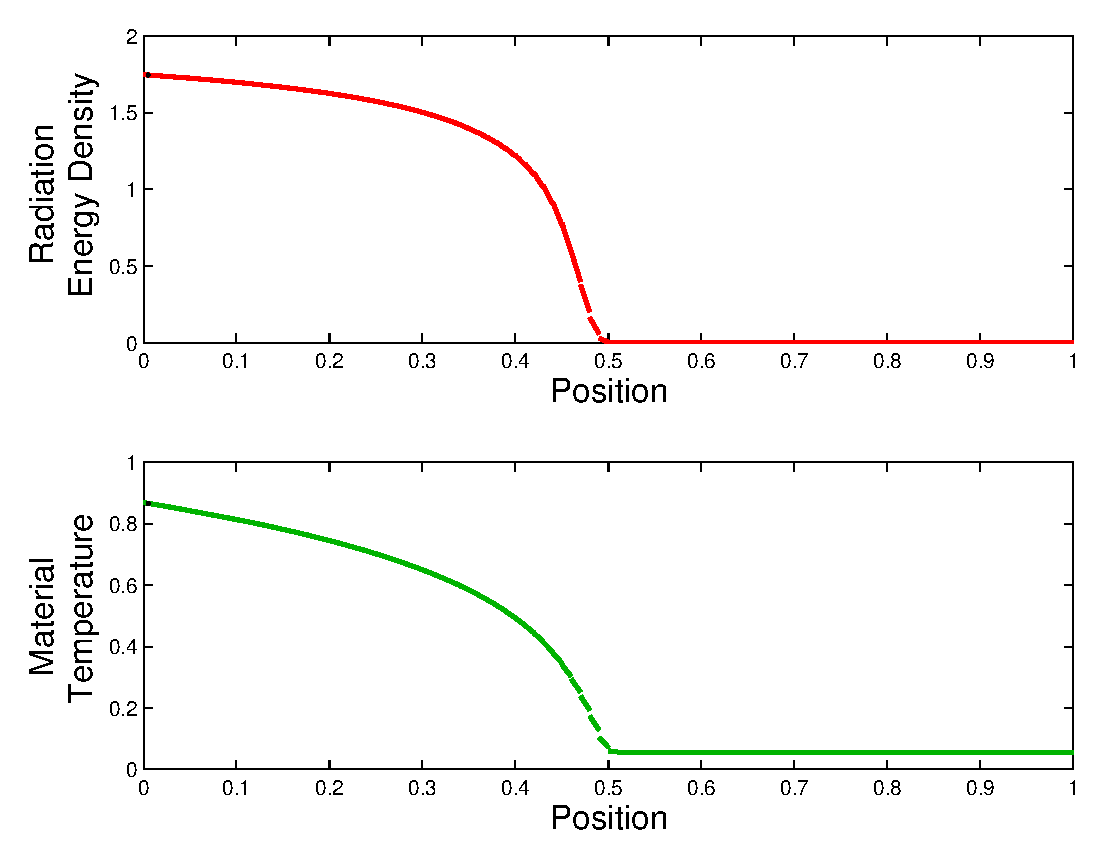
\includegraphics[width=10cm]{Proposal_ex_sol.eps}
\end{center}
\caption{Example solution of the Marshak wave problem.}
\label{fig:example}
\end{figure}
To obtain \fig{fig:example}, we used 100 mesh cells, a linear trial space, and self-lumping Lobatto quadrature that explicitly accounted for the variation of cross section in each cell.

We now demonstrate the effects of assuming a constant opacity in each cell.  
In \fig{fig:blades}, we use the same computational mesh, trial space, and lump the mass matrix, but assume a cell-wise constant opacity, equal to the cell average opacity.
\begin{figure}[!hbp]
\begin{center}
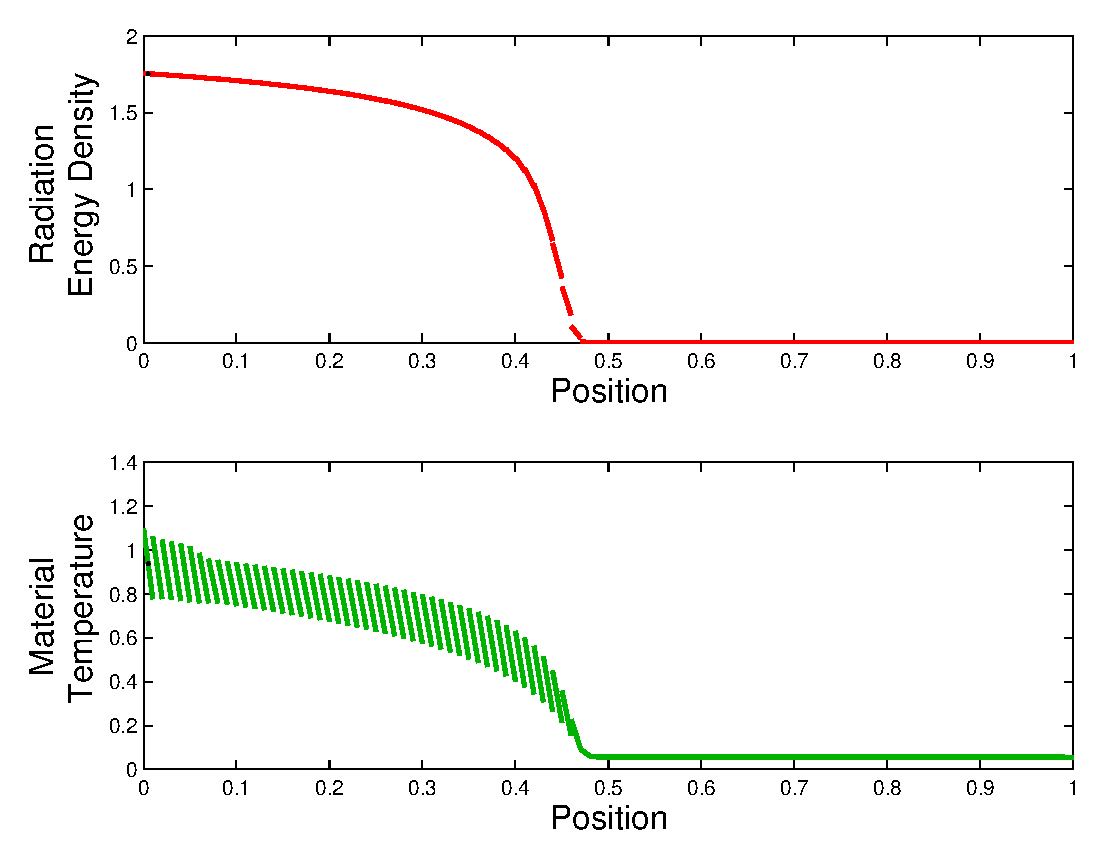
\includegraphics[width=10cm]{Proposal_blades.eps}
\end{center}
\caption{Lumped linear discontinuous solution assuming cell-wise constant opacity.}
\label{fig:blades}
\end{figure}
Obviously, the large, persistent non-monotonic discontinuities in the temperature profile are non-physical.  
However, this ``blading'' phenomena has gone unnoticed due to historical choices in data presentation.
If instead of presenting the true, discontinuous approximation of the temperature profile, as in \fig{fig:blades}, we plot cell average quantities at cell centers, the blading effect cannot be seen, as shown in \fig{fig:plot}.
\begin{figure}[!htp]
\begin{center}
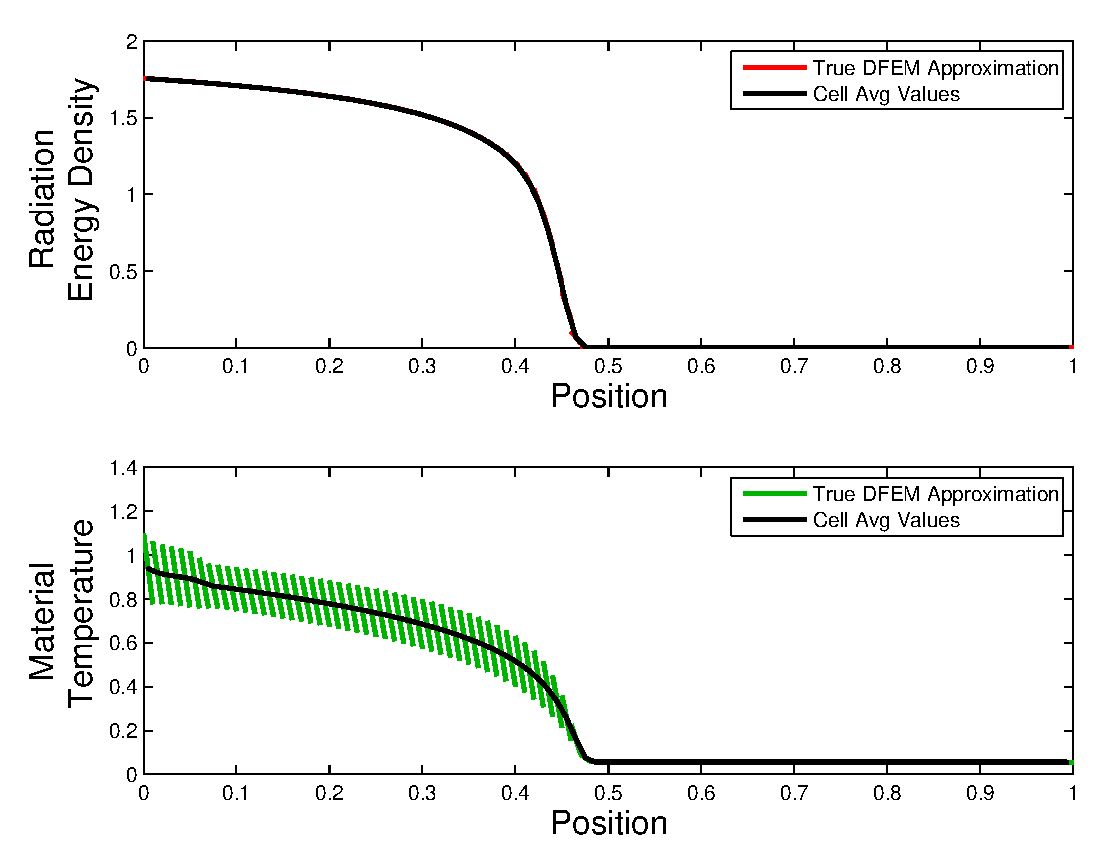
\includegraphics[width=10cm]{Proposal_plot.eps}
\end{center}
\caption{Constant opacity, lumped linear discontinuous DFEM approximation solution.  Comparison of cell averages interpolated at cell centers versus true discontinuous solution approximation.}
\label{fig:plot}
\end{figure}

The effects of using higher degree polynomial trial spaces for radiative transfer have also been explored using the grey Marshak wave test problem.
As an example, consider \fig{fig:ho_trt} that shows numerical results for DFEM schemes with different trial space degrees, but using the same total number of unknowns in each scheme.
\begin{figure}[!htp]
\begin{center}
\subfigure[60 Unknowns]{
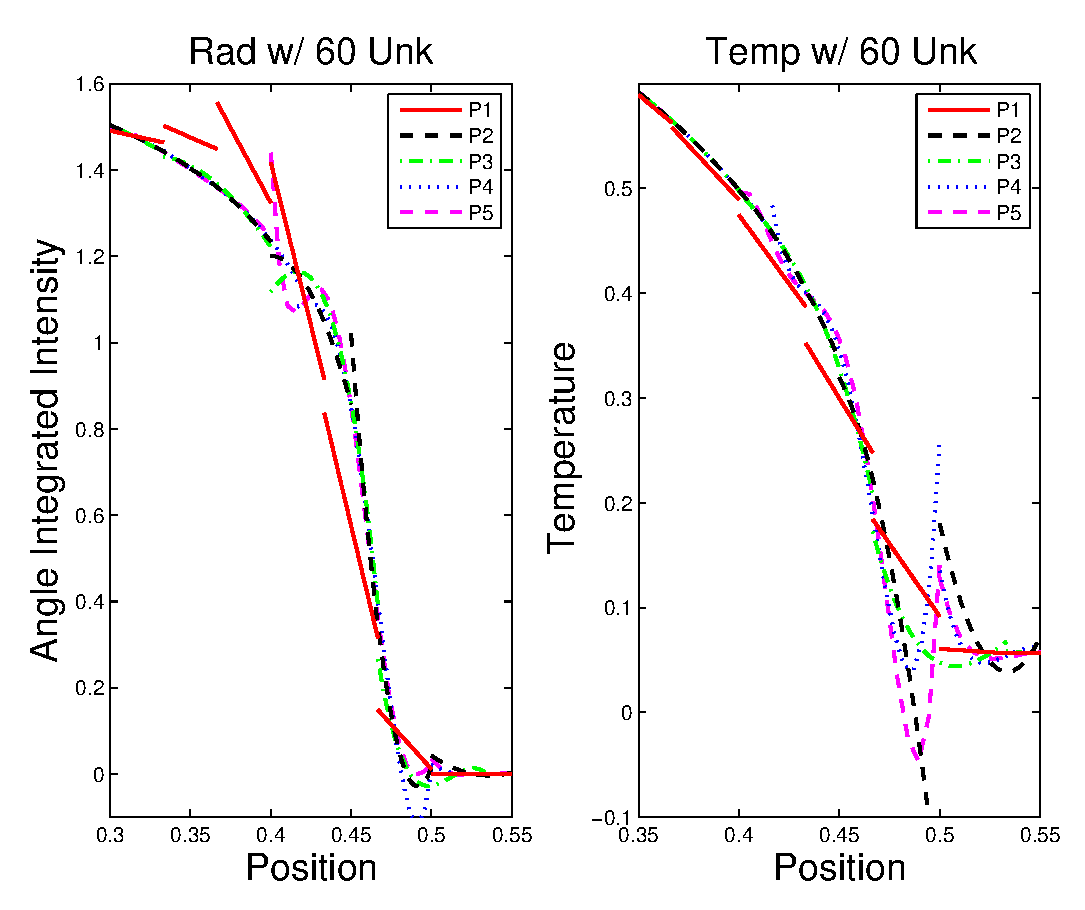
\includegraphics[width=11cm]{WaveFront_60_Unk.eps}
}
\subfigure[120 Unknowns]{
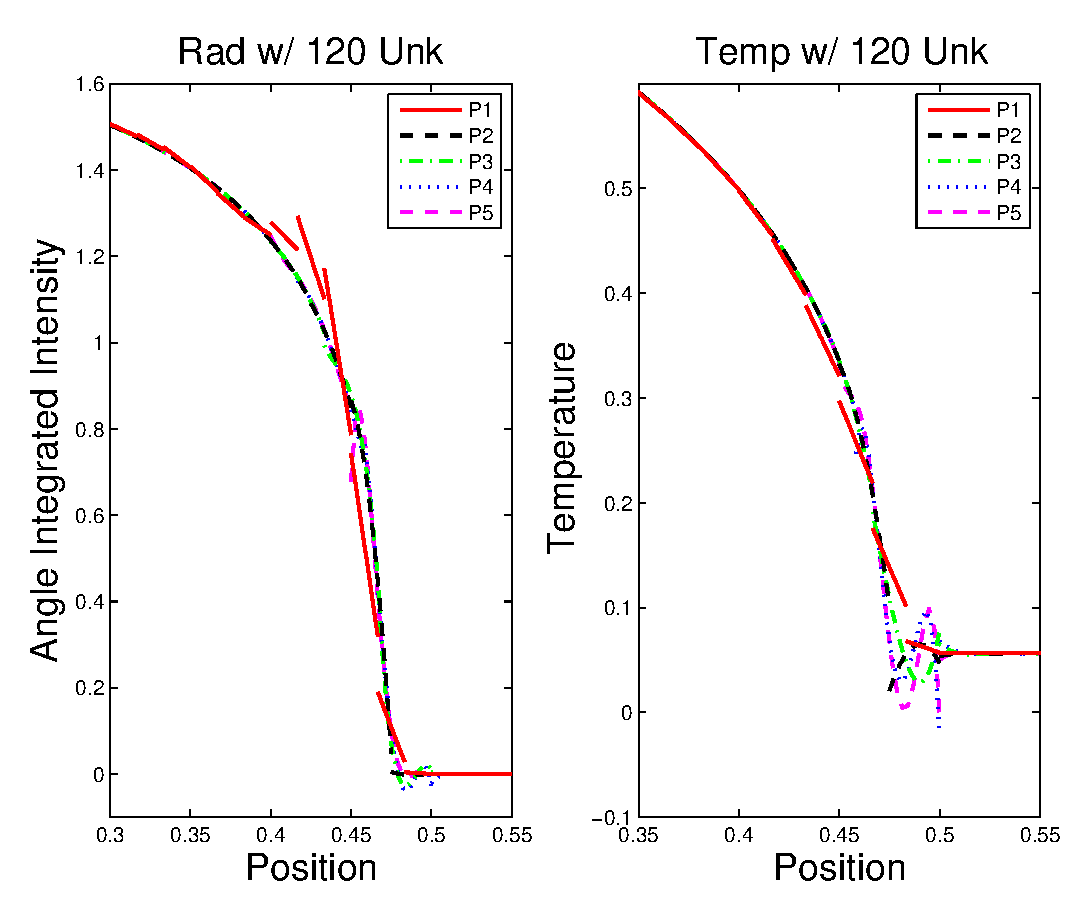
\includegraphics[width=11cm]{WaveFront_120_Unk.eps}
}
\end{center}
\caption{Comparison of numerical solutions at the wave front using the same total number of unknowns and different DFEM trial space degrees.}
\label{fig:ho_trt}
\end{figure}


%%%%%%%%%%%%%%%%%%%%%%%%%%%%%%%%%%%%%%%%%%%%%%%%%%%%%%%%%%%%%%%%%%
%%%%%%%%%%%%%%%%%%%%%%%%%%%%%%%%%%%%%%%%%%%%%%%%%%%%%%%%%%%%%%%%%%
\section{Future Work} 
%%%%%%%%%%%%%%%%%%%%%%%%%%%%%%%%%%%%%%%%%%%%%%%%%%%%%%%%%%%%%%%%%%
%%%%%%%%%%%%%%%%%%%%%%%%%%%%%%%%%%%%%%%%%%%%%%%%%%%%%%%%%%%%%%%%%%

To complete the project, we will use C++ to write a multi-frequency radiative transfer code.
The code will incorporate all of the work we have developed and implemented in the grey radiative transfer code: SDIRK time integration, arbitrary order DFEM, and self-lumping quadrature that accounts for the spatial variation of cross section in each cell using equally-spaced, Lobatto, or Gauss quadrature points.
We will use preconditioned Krylov methods, using both sweep and DSA \cite{mip_dsa} preconditioners, to iteratively solve the within group scattering problem.
Likewise, we will iterate on the absorption rate density using Krylov methods with LMFGA as in \cite{warsa_lmfga}.
The effectiveness and efficiency of a low order diffusion operator used to accelerate high order DFEM discretizations will be examined.
%We do not expect DSA/LMFGA using a LDFEM diffusion operator to necessarily be stable when used as a fixed point acceleration scheme.
%However, we are optimistic that when used as a Krylov preconditioner that the overall iteration scheme will be stable and effective.

The Trilinos code package \cite{trilinos} will be used to invert the diffusion operator.
Though the 1-D diffusion operator is block diagonal and can be directly inverted, using Trilinos offers direct solvers, iterative solvers, and the ability to use powerful preconditioners such as algebraic multi-grid.
Additionally, Trilinos has a GMRES Krylov solver that can be used to solve the scattering and absorption/re-emission iterations efficiently.

% How to Verify it's working?
Given the complexity of thermal radiative transfer, benchmark solutions are difficult to find.  
The most commonly used benchmarks come from the work of Su and Olson \cite{su_olson_1,su_olson_2}.
While the Su and Olson benchmarks offer analytic solutions that can be used for code verification, they are not ideal for comparing the relative accuracy or convergence rates of different numerical schemes.
To be used as convergence comparison tools requires that the analytic integrals in \cite{su_olson_1} and \cite{su_olson_2} be numerically evaluated to a very tight tolerance, a non-trivial task.
The Su and Olson benchmark solutions are given in terms of two-dimensional improper integrals with an integrand that is a composite function of a trigonometric function of a slowly decaying function.
Even with the use of advanced, recursive numerical techniques \cite{numerical_book}, the evaluation of the Su and Olson integrals for even a single state point, that is the temperature or radiation energy density at one point in space, at one instance in time is a computationally intense task.
Thus, using analytical benchmarks to measure and compare the accuracy of our different numerical schemes is not practical.

An alternative to using analytical solutions as a benchmarking tool is to use code-to-code comparisons.
One can use published results, for instance the results in \cite{morel_radtran}, but these comparisons are again of limited utility in determining order of convergence/relative accuracy of numerical methods.
The difficulty in using published results is that the results are not necessarily reproduced with their full accuracy, may have been found using limited tolerances, used non-comparable solution methodologies, or give only a few data points.
Like comparing against analytical results, comparison of our schemes to published numerical results of other schemes offers opportunities for validation, but is most likely insufficient for our purposes.

The most appropriate tool for quantifying our new methods' performance will be the Method of Manufactured Solutions (MMS) \cite{mms}.
By first defining a desired solution, then solving the analytic TRT equations assuming the manufactured solution, we generate an inhomogeneous driving source.
Using this manufactured source, we can then study the convergence of our methods to the manufactured solution.

Judging the effectiveness of our low order LMFGA acceleration technique/preconditioner is not as difficult as measuring the convergence and accuracy of our spatial discretization schemes.
To measure the effectiveness, we need data that is readily available: CPU timing data and iteration counts.
Using expert judgment, we will then choose different problems that have historically challenged iterative schemes.
We can then compare timing data and iteration counts to determine the efficiency and effectiveness of equal order DFEM DSA acceleration schemes to the respective values obtained using LDFEM diffusion operators.  

%%%%%%%%%%%%%%%%%%%%%%%%%%%%%%%%%%%%%%%%%%%%%%%%%%%%%%%%%%%%%%%%%%
%%%%%%%%%%%%%%%%%%%%%%%%%%%%%%%%%%%%%%%%%%%%%%%%%%%%%%%%%%%%%%%%%%

\section*{References}

\setlength{\baselineskip}{12pt}
\begin{thebibliography}{300}
%\bibitem{journal} B. Author(s), ``Title,'' {\it Journal Name in Italic}, 
%          {\bf Volume in Bold}, pp. 34-89 (19xx).
%\bibitem{proc_paper} C. D. Author(s), ``Article Title,'' {\it Proceedings of
%          Meeting in Italic}, Location, Dates of Meeting, Vol. n, pp. 134-156 
%          (19xx).
%\bibitem{book} E. F. Author, {\it Book Title in Italic}, Publisher, City \&
%          Country (19xx). 

\bibitem{reed} W. H. Reed and T. R. Hill and F. W. Brinkley and K. D. Lathrop, LA-5428-MS, Los Alamos National Lab, 1972 (unpublished).

\bibitem{larsen_nelson} E. W. Larsen and P. Nelson, ``Finite-Difference Approximations and Superconvergence for the Discrete Ordinates Equations in Slab Geometry,'' {\it SIAM Journal of Numerical Analysis}, {\bf 19 (2)} pp.334-348 (1982).

\bibitem{larsen_morel_asymptotics} E. W. Larsen and J. E. Morel, ``Asymptotic Solutions of Numerical Transport Problems in Optically Thick, Diffusive Regimes II,'' {\it Journal of Computational Physics}, {\bf 83} pp. 212-236 (1989).

\bibitem{morel_radtran} J. E. Morel and T. A. Wareing and K. Smith, ``A Linear-Discontinuous Spatial Differencing Scheme for $S_N$ Radiative Transfer Calculations,'' {\it Journal of Computational Physics}, {\bf 128} pp. 445-462 (1996).

\bibitem{walters} W. F. Walters, ``The Relation Between Finite Element Methods and Nodal Methods in Transport Theory,'' {\it Progress in Nuclear Energy}, {\bf 18}, pp. 21-26 (1986).

\bibitem{hennart_delvalle_2} J. P. Hennart and E. del Valle, ``A Generalize Nodal Finite Element Formalism for Discrete Ordinate Equations in Slab Geometry: Part II Theory in the Discontinuous Moment Case,'' {\it Transport Theory and Statistical Physics}, {\bf 24}, pp. 479-504 (1995).

\bibitem{hennart_delvalle_3} J. P. Hennart and E. del Valle, ``A Generalize Nodal Finite Element Formalism for Discrete Ordinate Equations in Slab Geometry: Part III Numerical Results,'' {\it Transport Theory and Statistical Physics}, {\bf 24}, pp. 505-533 (1995).

\bibitem{yaqi_ragusa} Y. Wang and J. C. Ragusa, ``On the Convergence of DGFEM Applied to the Discrete Ordinates Transport Equation for Structured and Unstructured Triangular Meshes'' {\it Nuclear Science and Engineering}, {\bf 163}, pp. 56-72 (2009).

\bibitem{warsa_prinja} J. S. Warsa and A. K. Prinja, ``p-adaptive Numerical Methods for Particle Transport,'' {\it Transport Theory and Statistical Physics}, {\bf 28(3)}, pp. 229-270 (1999).

\bibitem{adams} M. L. Adams, ``Discontinuous Finite Element Transport Solutions in Thick Diffusive Problems'', {\it Nuclear Science and Engineering}, {\bf 137}, pp. 298-333 (2001).

\bibitem{hamilton} S. Hamilton, M. Benzi, and J. Warsa, ``Negative Flux Fixups in Discontinuous Finite Elements SN Transport,'' {\it International Conference on Mathematics, Computational Methods \& Reactor Physics}, Saratoga Springs, New York, 3-7 May (2009). 

\bibitem{csz} P. Maginot, J. E. Morel, and J. Ragusa, ``A Non-negative Moment Preserving Spatial Discretization Scheme for the Linearized Boltzmann Transport Equation in 1-D and 2-D Cartesian Geometries,'' {\it Journal of Computational Physics}, {\bf 231(20)}, pp. 6801-6826 (2012).

\bibitem{lathrop} K. D. Lathrop, ``Spatial Differencing of the Transport Equation: Positivity vs. Accuracy,'' {\it Journal of Computational Physics}, {\bf 4}, pp. 475-498 (1969).

\bibitem{raviart} P. A. Raviart, ``The Use of Numerical Integration in Finite Element Methods for Solving Parabolic Equations,'' {\it Conference on Numerical Analysis, RIANA 1972}, Dublin, Ireland, 14-18 August, pp. 233-264 (1972).

\bibitem{thomee} V. Thomee, {\it Galerkin Finite Element Methods for Parabolic Problems}, Springer, New York (1997). 

\bibitem{abramowitz} M. Abramowitz and I. A. Stegun, {\it Handbook of Mathematical Functions with Formulas, Graphs, and Mathematical Tables}, United States Department of Commerce, Washington, D.C. (1972).

\bibitem{xs_are_T_dependent} W. M. Stacey, {\it Nuclear Reactor Physics}, John-Wiley \& Sons Inc. , New York, NY (2001).

\bibitem{lewis_book} E. E. Lewis and W. F. Miller, {\it Computational Methods of Neutron Transport},American Nuclear Society,	La Grange Park, IL (1993).

\bibitem{warsa_krylov} J. S. Warsa and T. A. Wareing and J. E. Morel, ``Krylov Iterative Methods and the Degraded Effectiveness of Diffusion Synthetic Acceleration for Multidimensional $S_N$ Calculations in Problems with Material Discontinuities,'' {\it Nuclear Science and Engineering}, {\bf 147(3)}, pp. 218-248 (2004).

\bibitem{varXS_diff} A. Kavenoky and J. Lautard, ``A Finite Element Depletion Diffusion Calculation Method with Space-Dependent Cross Section,'' {\it Nuclear Science and Engineering}, {\bf 64(2)}, pp.563-575 (1977).

\bibitem{varXS_MOC} S. Santandrea and P. Bellier, ``An Unstructured Characteristics Scheme With a Linear Expansion For Both Fluxes and Cross Sections,'' {\it Proceedings of the Joint International Topical Meeting on Mathematics \& Computation and Supercomputing in Nuclear Applications (M\&C + SNA 2007)}, Monterey, California, April 2007.

\bibitem{adams_scb} M. L. Adams, ``Subcell Balance Methods for Radiative Transfer on Arbitrary Grids,'' {\it Transport Theory and Statistical Physics}, {\bf 26}(4\&5), pp. 385-431 (1997).

\bibitem{adams_nowak} M. L. Adams and P. F. Nowak, ``Asymptotic Analysis of a Computational Method for Time- and Frequency- Dependent Radiative Transfer,'' {\it Journal of Computational Physics}, {\bf 146}, pp. 366-403 (1998).

\bibitem{ober_shadid} C. C. Ober and J. N. Shadid, ``Studies on the Accuracy of Time-Integration Methods for the Radiation-Diffusion Equations,'' {\it Journal of Computational Physics}, {\bf 195}, pp. 743-772 (2004).

\bibitem{warsa_lmfga} J. E. Morel and T.-Y. B. Yang and J. S. Warsa, ``Linear Multifrequency-Grey Acceleration Recast for Preconditioned Krylov Iterations,'' {\it Journal of Computational Physics}, {\bf 227}, pp. 244-264 (2007).

\bibitem{first_lmfga} J. E. Morel and E. W. Larsen and M. K. Matzen, ``A Synthetic Acceleration Scheme for Radiative Diffusion Calculations,'' {\em Journal of Quantitative Spectroscopy and Radiative Transfer}, {\bf 34 (3)}, pp. 243-261 (1985).

\bibitem{old_dsa} E. M. Gelbard and L. A. Hageman, ``Synthetic Methods As Applied to $S_N$ Equations'', {\em Nuclear Science and Engineering}, {\bf 37(2)}, pp. 288-298 (1969).

\bibitem{larsen_dsa} E. W. Larsen, ``Unconditionally Stable Diffusion-Synthetic Acceleration Methods for the Slab Geometry Discrete Ordinates Equations,'' {\it Nuclear Science and Engineering}, {\bf 82} pp. 47-63 (1982).

\bibitem{adams_dsa} M. L. Adams and W. R. Martin, ``Diffusion Synthetic Acceleration of Discontinuous Finite Element Transport Iterations,'' {\em Nuclear Science and Engineering}, {\bf 111}, pp. 145-167 (1992).

\bibitem{wwm_dsa} J. S. Warsa and T. A. Wareing and J. E. Morel, ``Fully Consistent Diffusion Synthetics Acceleration of Linear Discontinuous $S_N$ Transport Discretization on Unstructured Tetrahedral Meshes,'' {\it Nuclear Science and Engineering}, {\bf 141}, pp. 236-251 (2002).

\bibitem{wla_dsa} T. A. Wareing and E. W. Larsen and M. L. Adams, ``Diffusion Accelerated Discontinuous Finite Element Schemes for the $S_N$ Equations in Slab and X-Y Geometries,'' {\it Advances in Mathematics, Computations, and Reactor Physics}, Pittsburgh, Pennsylvania, April 28-May 2 (1991).

\bibitem{mip_dsa} Y. Wang and J. C. Ragusa, ``Diffusion Synthetic Acceleration for High-Order Discontinuous Finite Element $S_N$ Transport Schemes and Application to Locally Refined Unstructured Meshes,'' {\it Nuclear Science and Engineering} {\bf 166}, pp. 145-166 (2010).

\bibitem{mip_mc} B. Turcksin and J. C. Ragusa, ``A Diffusion Synthetic Acceleration Scheme for Rectangular Geometries Based on Bilinear Discontinuous Finite Elements,'' {\it International Conference on Mathematics and Computational methods, Applied to Nuclear Science and Engineering}, Sun valley, Idaho, 5-9 May (2013).

\bibitem{mc_2013} P. G. Maginot and J. C. Ragusa and J. E. Morel, ``Characterization of High Order Spatial Discretizations and Lumping Techniques for Discontinuous Finite Element $S_N$ Transport,'' {\it International Conference on Mathematics and Computational methods, Applied to Nuclear Science and Engineering}, Sun valley, Idaho, 5-9 May (2013).

\bibitem{part_1_paper} P. G. Maginot and J. C. Ragusa and J. E. Morel, ``Lumping Techniques for DFEM Transport in $S_N$ Transport in Slab Geometry,'' {\it Nuclear Science and Engineering}, {\it (in final submission)} (2014).

\bibitem{part_2_paper} P. G. Maginot and J. C. Ragusa and J. E. Morel, ``Accurate Methods for DFEM $S_N$ Transport in Slab Geometry for Non-piecewise Constant Cross Section Problems,'' {\it Annals of Nuclear Energy}, {\it (in submission) } (2014).

\bibitem{trilinos} M. Heroux, et al, ``An Overview of Trilinos,'' ``Sandia National Laboratories Technical Report,'' SAND2003-2927 (2003).

\bibitem{su_olson_1} B. Su and G. L. Olson, ``An Analytical Benchmark for Non-Equilibrium Radiative Transfer in an Isotropically Scattering Medium,'' {\em Annals of Nuclear Engergy}, {\bf 24(13)}, pp. 1035-1055 (1997).

\bibitem{su_olson_2} B. Su and G. L. Olson, ``Non-Grey Benchmark Results for Two Temperature Non-Equilibrium Radiative Transfer,'' {\em Journal of Quantitative Spectroscopy and Radiative Transfer}, {\bf 62} pp. 279-302 (1999).

\bibitem{numerical_book} W. H. Press and S. A. Teukolsky and W. T. Vetterling and B. P. Flannery, Numerical Recipes in FORTRAN, 2nd Edition, Cambridge University Press, New York, 1992.

\bibitem{mms} K. Salari and P. Knupp, ``Code Verification by the Method of Manufactured Solutions,'' {\it SANDIA Technical Report}, SAND2000-1444 (2000).

\end{thebibliography} 


\end{document}


